%!TEX root = /Users/andcj/Dropbox/Documents/PhD/Thesis/phdthesis.tex
\chapter{Telescope design for the International AXion Observatory (IAXO)}\label{chap:iaxo}
CAST is a third generation axion helioscope and was the first experiment to surpass the astrophysical limit on the axion-photon coupling of \gay\ $\lesssim 10^{10}$ Gev$^{-1}$ in a broad axion mass range. The CAST helioscope search has reached slightly into the part of parameter space predicted by models to be most likely to detect the axion.

To improve on the CAST achievements and reach further into the \emph{axion band} of the parameter space, a more sensitive instrument is required.

\section{IAXO concept}
Considering that the probability of converting a solar axion into a photon in a magnet with magnetic field $B$ and length $L$ is given by\cite{Andriamonje:2007jc,Zioutas:2005jl,Sikivie:1983wx}:

\begin{eqnarray}
  P_{\text{a}\gamma} &=& 2.6\cdot10^{-17}\bigg(\frac{B}{10\text{ T}}\bigg)^2\bigg(\frac{L}{10\text{ m}}\bigg)^2(g_{\text{a}\gamma}\cdot10^{10}\text{\ GeV})^2\mathcal{F},
\end{eqnarray}

where $\mathcal{F}$ is the coherence length:

\begin{eqnarray}
  \mathcal{F} &=& \frac{2(1-\cos{qL})}{(qL)^2}
\end{eqnarray}

and $q$ is the momentum transfer. It becomes apparent that in order to improve on the probability of axion-photon conversion, either $B$ or $L$ has to be improved. In CAST $B \leq 9$ T, and it is already the limit of what is achievable with a large superconducting magnet. The magnet could be made longer, but it also has to be able to point at the sun and the improvement will only be a factor of two for a magnet twice as long. The last possibility is to increase the collecting area of the magnet, so instead of two bores of 43 mm diameter like in CAST, bore diameter could be prioritised over magnetic field. An optimal design for a new magnet was identified\cite{Irastorza:1340820} in the ATLAS magnet for LHC\cite{Collaboration:1997vu}, since it achieves a much larger cross section area by having much larger bores.

Using the toroidal design of the ATLAS magnet, a proposed design gave a magnet 25 m long with a peak magnetic field of $B \leq 5.4$ T. Using eight one meter wide and 21 m long racetrack coils. The magnet bores would be each 600 mm diameter and could be placed either inside the coils or between them. A higher magnetic field could be achieved by placing the bores inside the coils, but the coils would themselves block converted X-ray photons from reaching the detector (fig. \ref{fig:toroid_field}). Eight magnet bores of 25 m length, 600 mm diameter and $B \leq 5.4$ T, would equal approximately the same $BL$ as CAST, but achieving a cross section area of $\sim2.3$ m$^2$ compared to $3\cdot10^{-3}$ m$^2$ for CAST.

\begin{figure}[!h]
  \center
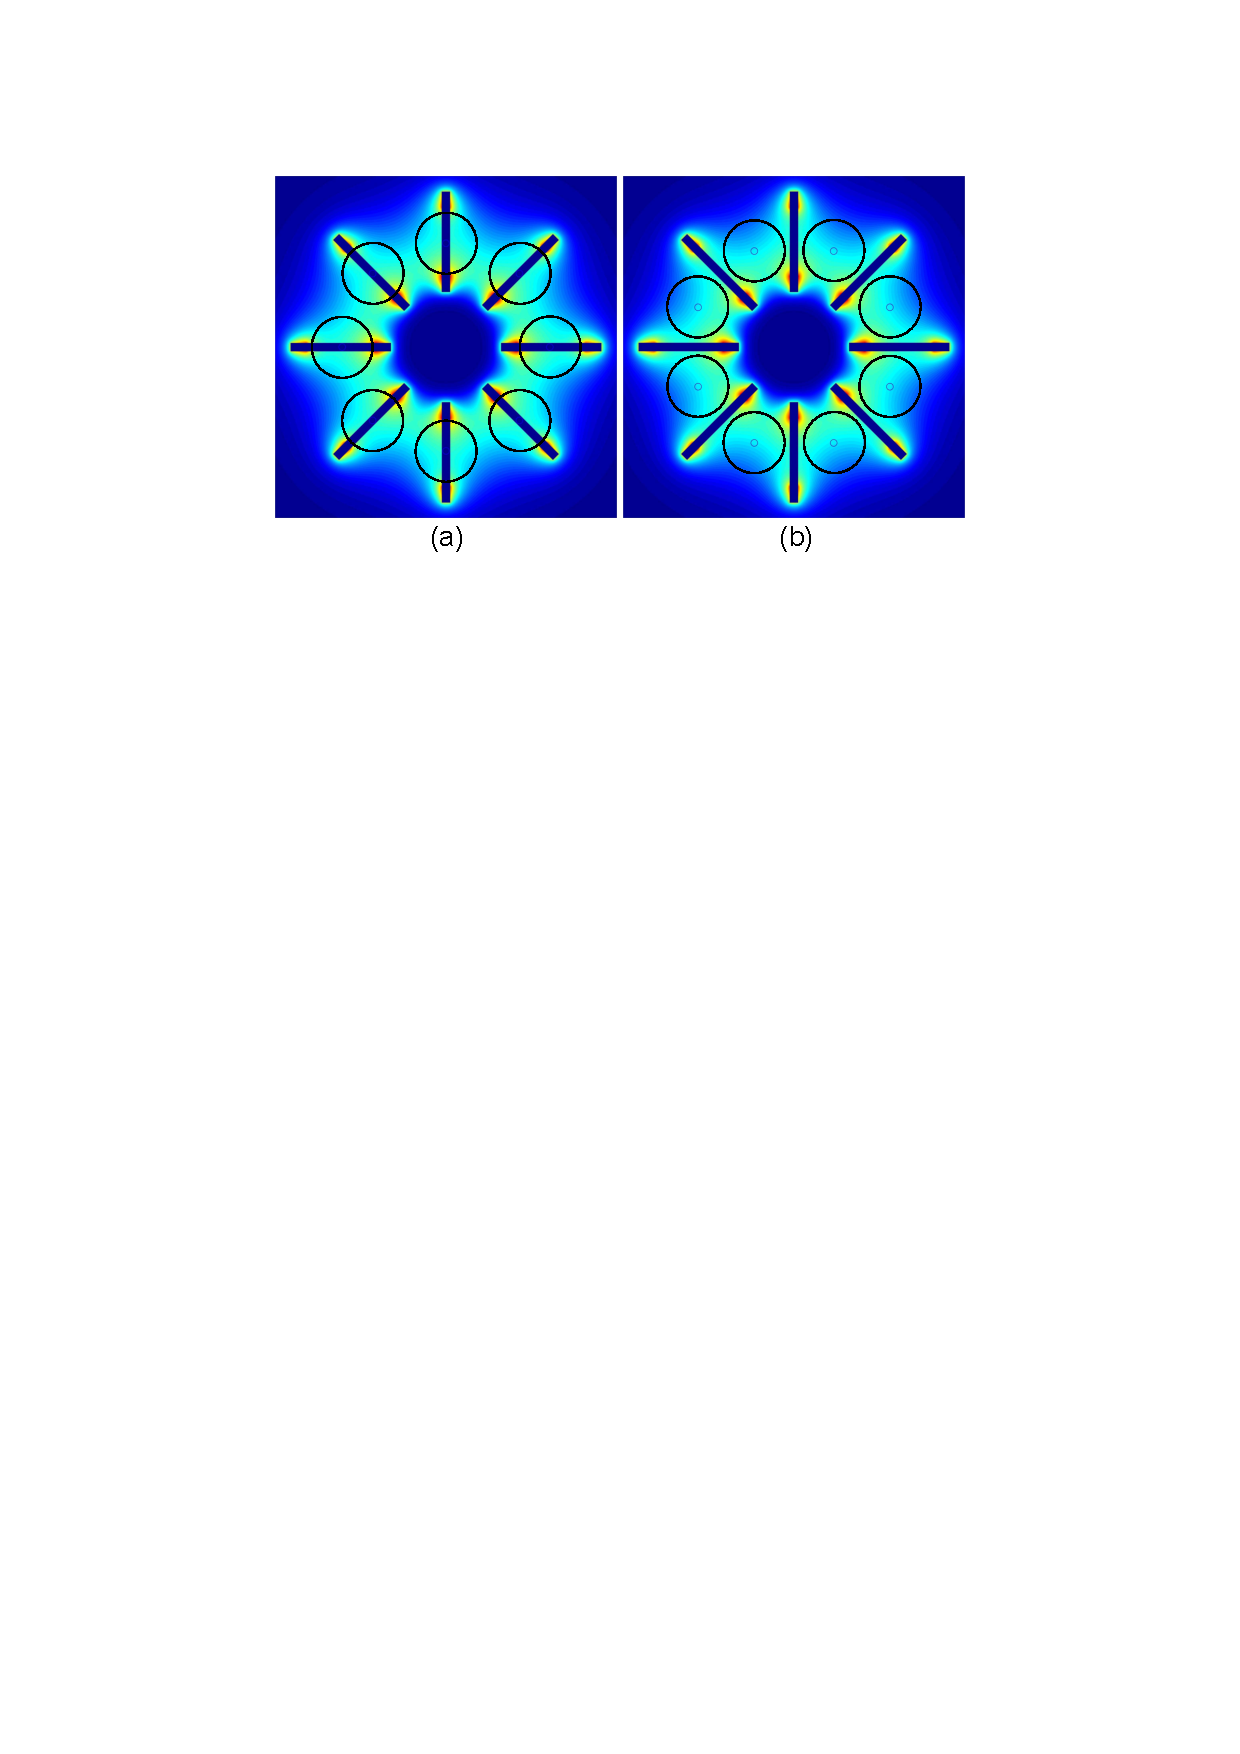
\includegraphics[width=0.8\linewidth]{figures/iaxo/toroid_field.pdf}
\caption{\footnotesize Illustration of the bore configurations with respect to superconducting coils in the IAXO magnet. Having the bores inside the coils (a) will give a stronger magnetic field, but X-ray telescopes at the end of each bore will be blocked in the center by the coil. With the bores between the coils (b), the magnetic field is not as strong, but the entire bore cross section area is usable. From \cite{Irastorza:2013uu}.}\label{fig:toroid_field}
\end{figure}

The large cross section will require X-ray telescopes to focus converted X-ray photons into detectors, as low-background detectors with such a large collecting area would not be possible. A design of the IAXO helioscope\cite{Vogel:2013we,Shilon:1501687,Irastorza:2012tt} with X-ray telescopes at each magnet bore can be seen in figure \ref{fig:iaxo_helioscope}. The proposed design of IAXO can achieve much higher inclination than CAST ($\pm$25\degr\ vs. $\pm$8\degr), so will be able to follow the sun for longer periods ever day.

\begin{figure}[!h]
  \center
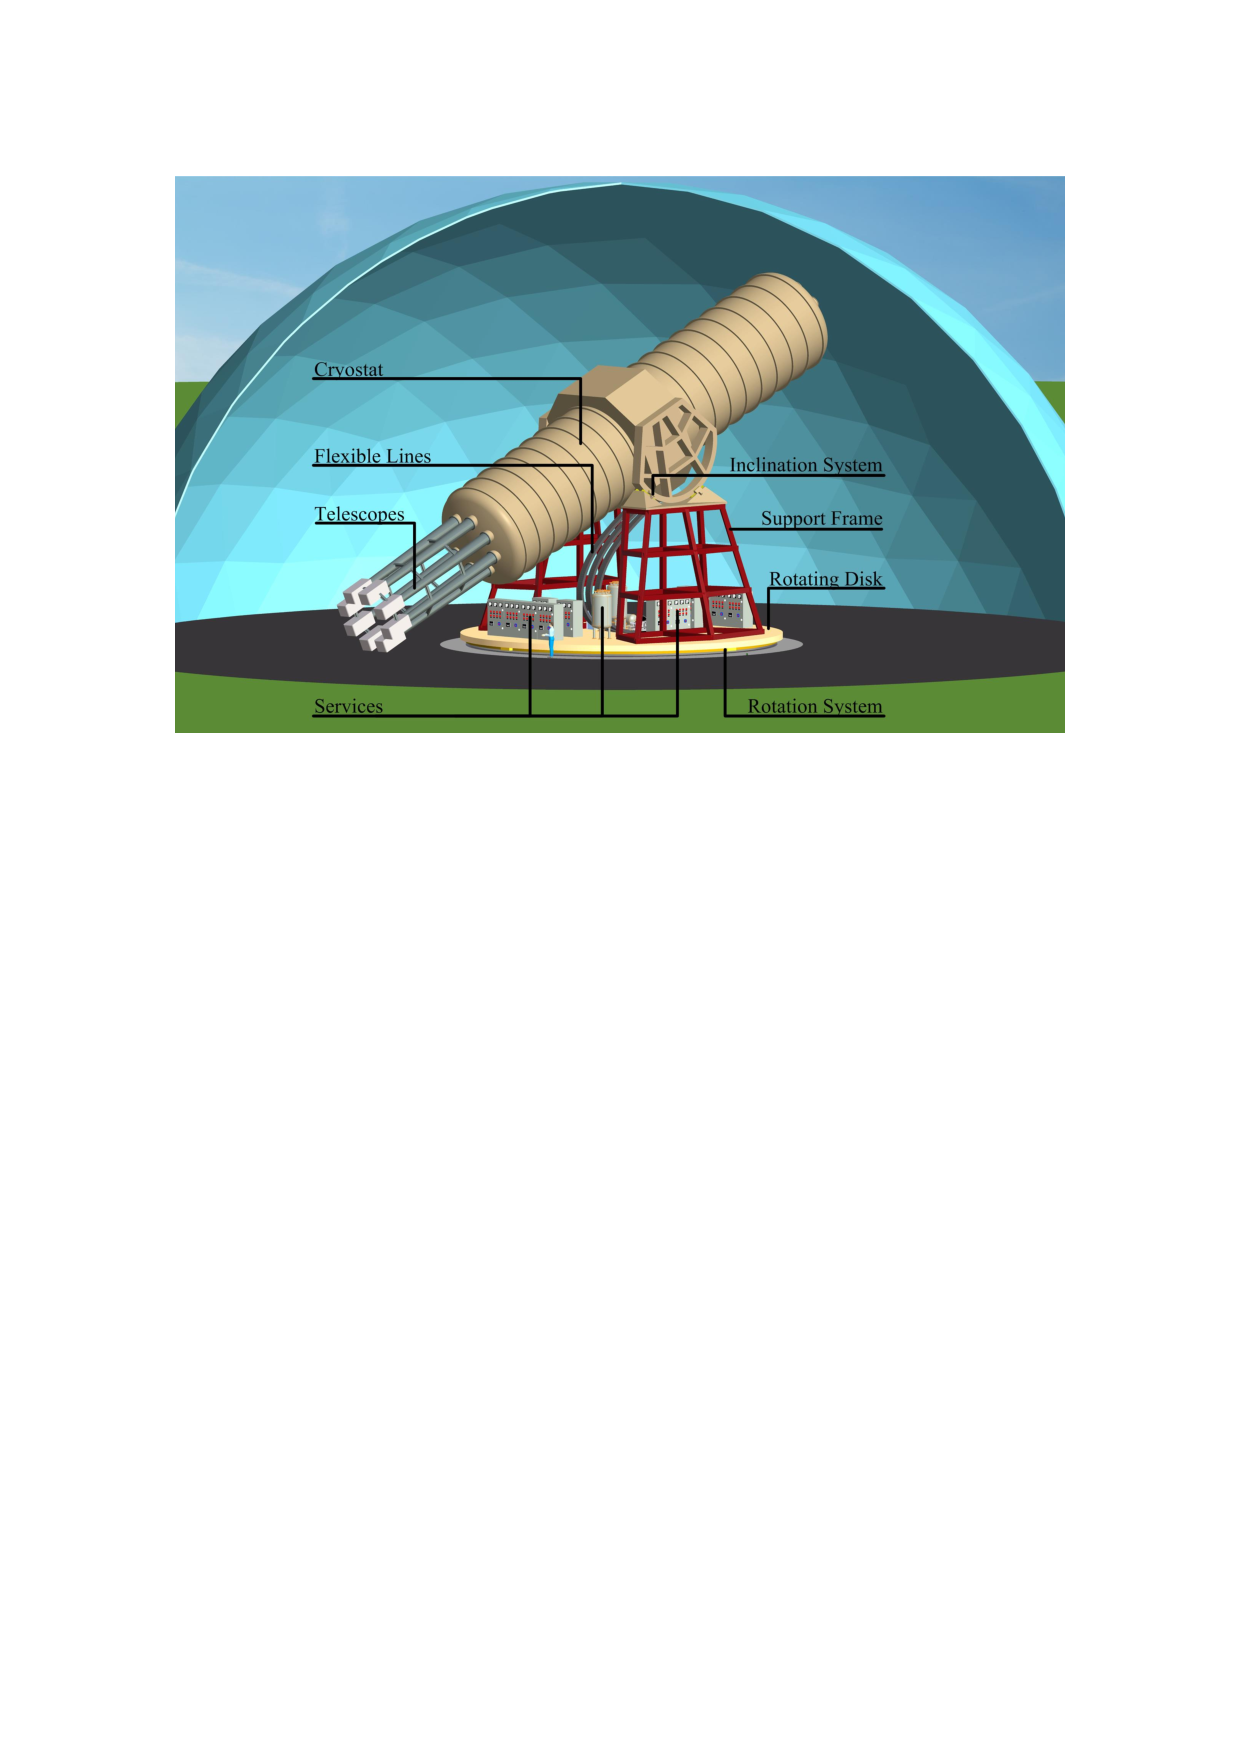
\includegraphics[width=0.8\linewidth]{figures/iaxo/iaxo_helioscope.pdf}
\caption{\footnotesize Schematic view of the IAXO helioscope. The cryostat containing the toroidal superconducting magnet is placed on a turret with complete 360\degr\ of rotation. Eight telescopes with separate detectors are placed at the end. Flexible lines feeds the magnet with liquid He and power. A fixed dome can cover the whole experiment as axions will not interact with the walls. From \cite{Armengaud:2014eo}.}\label{fig:iaxo_helioscope}
\end{figure}

IAXO will be able to achieve a sensitivity five orders of magnitude better than CAST, which translates into \gay values as low as $\sim5\cdot10^{-12}$ GeV$^{-1}$ for axion masses up to $\sim$0.01 eV, as can be seen in figure \ref{fig:iaxo_search}. The experiment would explore deep into the ALP\footnote{Axion-like particle} and axion parameter space, and even without detection would exclude a large region of QCD axion phase space that is completely unexplored. A detection of any fundamental pseudo-scalar particle would be groundbreaking for particle physics.

\begin{figure}[!h]
  \center
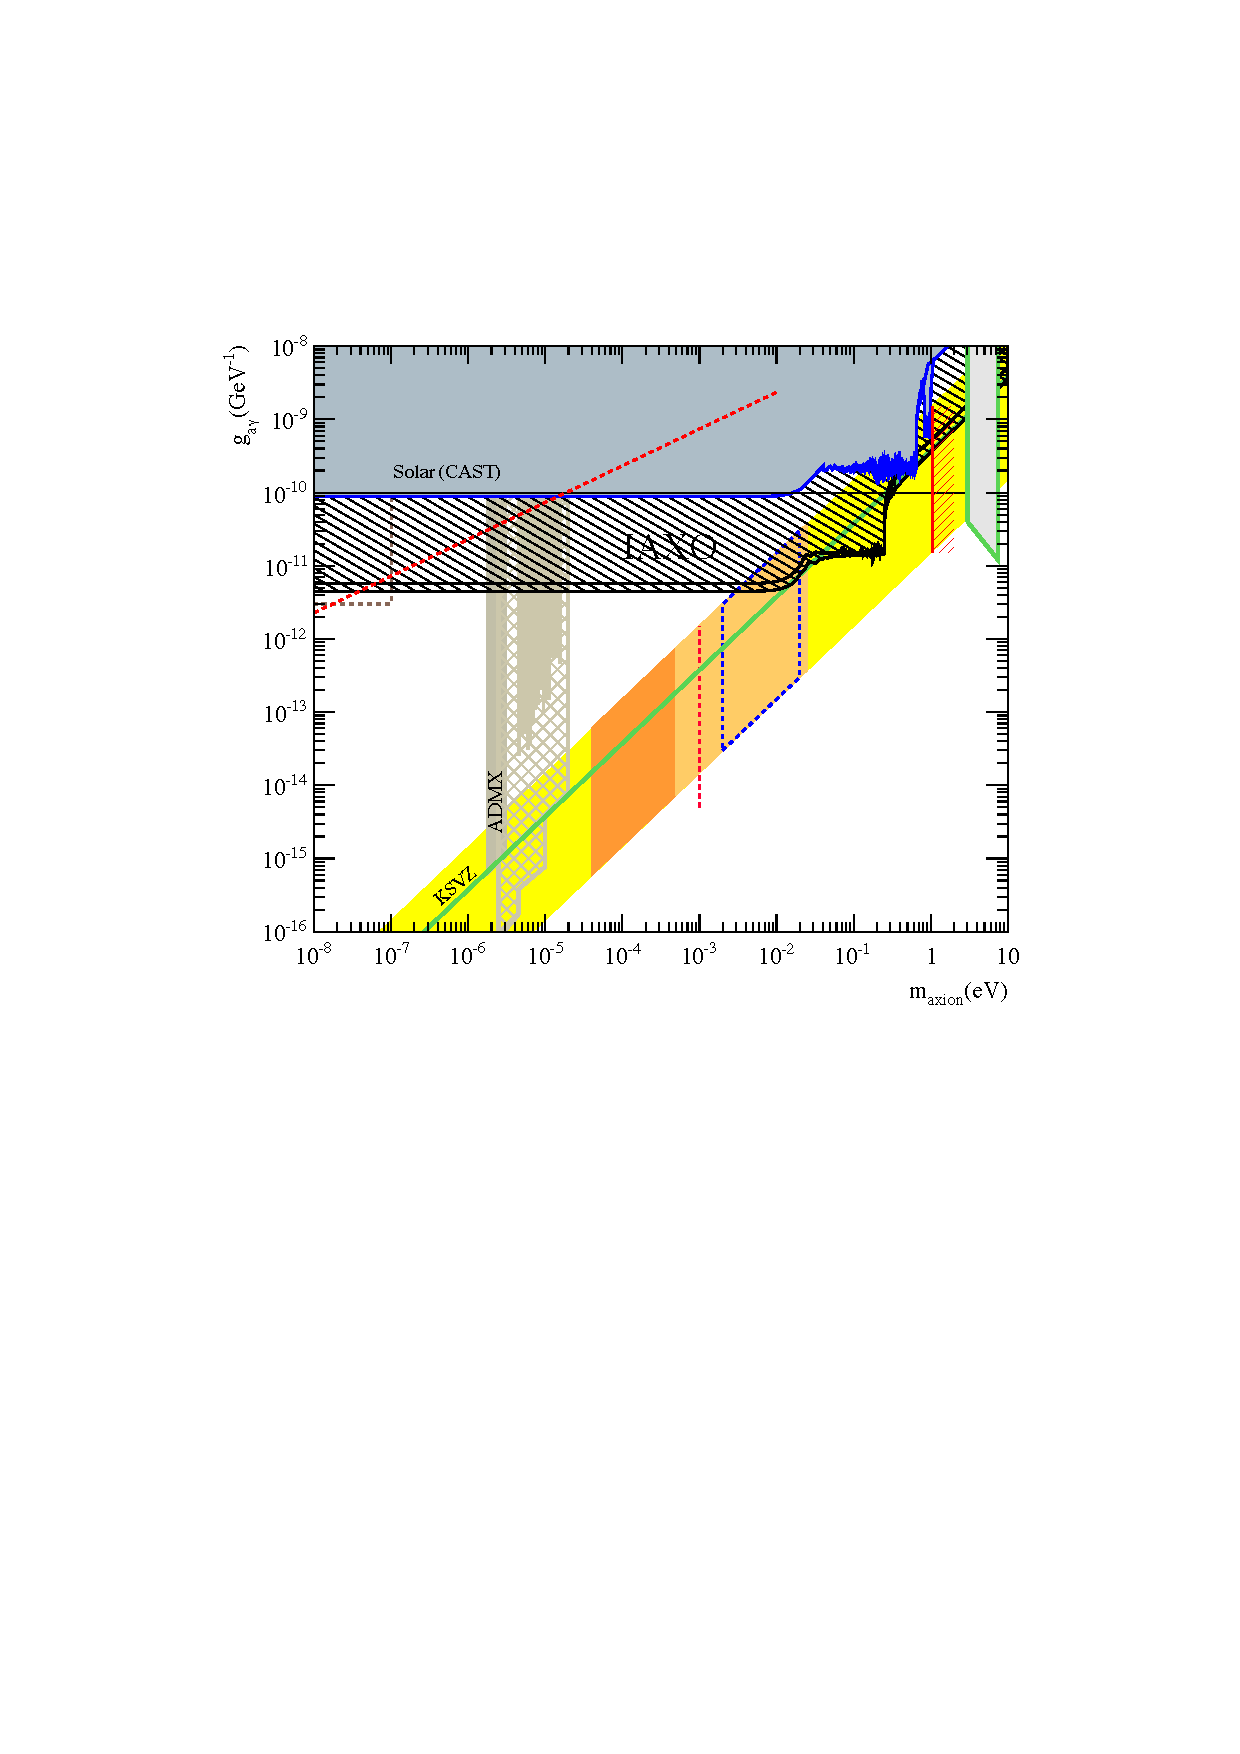
\includegraphics[height=8.5cm]{figures/iaxo/iaxo_axion_search.pdf}
\caption{\footnotesize The expected sensitivity of IAXO with currently excluded regions by CAST and ADMX\cite{Asztalos:2001ty} shown. Refer to fig. \ref{fig:axion_search_cast} for labels of the various regions. From \cite{Irastorza:2013uu}.}\label{fig:iaxo_search}
\end{figure}

\section{X-ray telescope design}
In appendices \ref{pap:iaxo_concept}, and to some extent \ref{pap:axion_spie}, the design of X-ray telescopes for IAXO is described in detail. Using a modified version of the software developed for the CAST optic, a geometry for a NuSTAR-like optic was found.

The IAXO helioscope will be without the limitations in telescope focal length found in the CAST experiment. The design of the telescope should however take into consideration the focal spot size resulting from the optic figure error and angular size of the sun. A longer focal length will increase the throughput of the optic, but will also increase the spot size. An algorithm for optimising the focal length was developed, and a 5 m focal length was found to be the optimal solution.

An additional outcome of the shorter focal length is the easier production demands as a result of fewer glass substrate layers in the optic. A 10 m focal length would require 235 glass substrate layers, compared to 133 layers for NuSTAR which has a similar focal length but only 400 mm diameter. With eight telescopes, that would result in $\sim8,000\cdot8=64,000$ glass substrates for IAXO, which is a large undertaking considering that the coating of $\sim6,000$ glass substrates for NuSTAR took a year full time at the DTU Space coating facility. The 5 m focal length would only require 110 glass substrate layers; it would also put less demand on the structure of vacuum tubes going from telescopes to detectors (see figure \ref{fig:iaxo_helioscope}).

\section{Coatings for IAXO X-ray telescopes}
Eight telescopes with 110 glass substrate layers is still a large undertaking for the coating chamber at DTU Space. The coating of all glass substrates would not be achievable in the 2.5 year time span set by the Letter of Intent\cite{Irastorza:2013uu} submitted to CERN in 2013. New coating chamber(s) would be needed and a year is set aside for the setup of new coating facilities before production begins.

For a large-scale coating production on curved glass substrates, a departure from the design of the coating facility at DTU Space is required. One of the main drawbacks is the inability to change samples for coating without opening the chamber completely. After closing the chamber with new samples inside, five to six hours of pumping is required in order to achieve the base pressure of $\leq 2\cdot10^{-6}$ Torr. A NuSTAR like coating that takes 12 hours to coat, requires 18 hours after samples are put into the chamber before they are completely coated. A load lock system would be able to almost remove the pump-down time.

The coatings for IAXO are similar to CAST and Athena coatings, 5--15 bilayers of 5--20 nm d-spacing, so each coating is relatively quick. The coating chamber at DTU Space has a rotational geometry, an advantage when coating many ($>100$) bilayers, but that is not required for IAXO. Instead it is advantageous to make a linear coating system, where substrates are placed on $\sim$60x60 cm$^2$ horizontal sample holder plates and the plates are stacked in a hopper-like system. A hopper with 10 plates each holding 6--8 samples could be placed in a load-lock and the system would automatically take out the plates to be coated one at a time. The plates would move horizontally past a number of cathodes, where one layer would be deposited on the way out and one layer on the way back, resulting in one bilayer per return trip. Each plate can be applied a different coating based on the velocity of the plate across the cathode plasma and the cathode power setting. The number of bilayers is set by the number of return trips of a plate.

The cathodes should be linear magnetrons of $\sim$80 cm length, placed horizontally and pointing down. Increased uniformity of coating on the cylindrically curved substrates that would be used for IAXO can be achieved by measuring the curvature of each sample in the chamber immediately before coating using a distance sensor. The cathodes could then automatically increase/decrease power as the samples move by according to the curvature of each sample.

Using two chambers of the design proposed above, the $\sim$30,000 substrates can be coated within the two year time span set by the Letter of Intent.

\section{IAXO conclusion}
In this chapter was described shortly the considerations taken in the design of X-ray telescopes for IAXO. Using a modified version of the software used to design the CAST XRT, telescopes suitable for IAXO were designed and an optimal focal length of 5 m were found.

IAXO is an international collaboration involving 29 institutes from across the world, each playing a part in the design, construction and operation of the experiment. The main barrier at the time of writing is the funding of the $\sim$100M \euro\ experiment, but both European and American institutions and agencies have expressed their interest in the project.

The Letter of Intent for IAXO, submitted in 2013, was approved by CERN in spring of 2014 making IAXO an official experiment at CERN. The IAXO collaboration was encouraged by CERN to take the next steps toward a technical design report that would include R\&D on magnet, detectors and X-ray telescopes.
